\RequirePackage{plautopatch}
\documentclass[dvipdfmx,a4paper]{jsarticle}
\usepackage{amsmath}
\usepackage{amssymb}
\usepackage[dvipdfmx]{graphicx}
\usepackage[margin=20truemm]{geometry}
\usepackage{url}
\usepackage{wrapfig}
% for hyperref
\usepackage[dvipdfmx, bookmarkstype=toc, colorlinks=false, pdfborder={0 0 0}, bookmarks=true, bookmarksnumbered=true]{hyperref}
\usepackage{pxjahyper}
\usepackage{here}

\title{\vspace{-1cm}テクニカルドキュメント}
\author{\texttt{こんぶ畑}}
\date{2024年3月1日}

\begin{document}

  \maketitle
  \section{チーム基本情報}
    
    \subsection{チームコード・チーム名}
    WRS002 こんぶ畑
    \subsection{リーグ}
    Rescue Simulation (Erebus)
    \subsection{国・地域}
    岡山

  \section{チーム情報}
    \subsection{チームについての説明}
    \noindent
    チーム名:こんぶ畑 (こんぶばたけ)

    \noindent
    メンバーの 1 人が所属していた部活の愛称と顧問への敬意を込めて名付けた。\\
    リーダー は高 1、高 2 とレスキューラインに参加してきた。今年度は受験の年で参加は半ば諦めていたが、幸運にも年内に志望校合格を果たし、もう 1 人を連れてくることでチームを結成することができた。\\
    結成は2024年になってからだ。わずか3ヵ月で初めての競技に挑む。

    \subsubsection{情報公開}
    \noindent
    情報公開はロボカップジュニアの国是のようなもだ。\\
    しかし、シミュレーションリーグでコードをオープンにすることは、実機リーグのそれとは持つ意味合いが少し違うと考える。良くも悪くも、たった 1 つの exe ファイルが文字通り「全て」なのだから。だが、RCJJ のコミュニティに何か少しでも貢献できることがあればと思い、今年もソースコードを大会終了後にGitHubで公開することにした。\href{https://github.com/KOMBU-Batake}{リンク}\\
    実際にこのソースコードを公開することで直接誰かの参考になるとはあまり思っていない。それよりも、自分を含めより多くの人が情報公開をすることで、よりコミュニティが活発になることに期待している。

    \subsection{チームの所属団体}
    \noindent
    個人参加

    \subsection{チームメンバー}
    \noindent
    ○○○○(●●●●)\\
    リーダーとしてプログラムの作成をした。\\
    今年こそ最後の大会。悔いのないように頑張りたい。\\

    \vskip.5\baselineskip
    \noindent
    □□□□(■■■■)\\
    突然誘われた一般人\\
    プログラム関連は無知\\
    フィールド作成、ポスターのデザイン提案、修正を行った。
  
  \section{ロボットの構成}
    \subsection{ロボットの写真}
    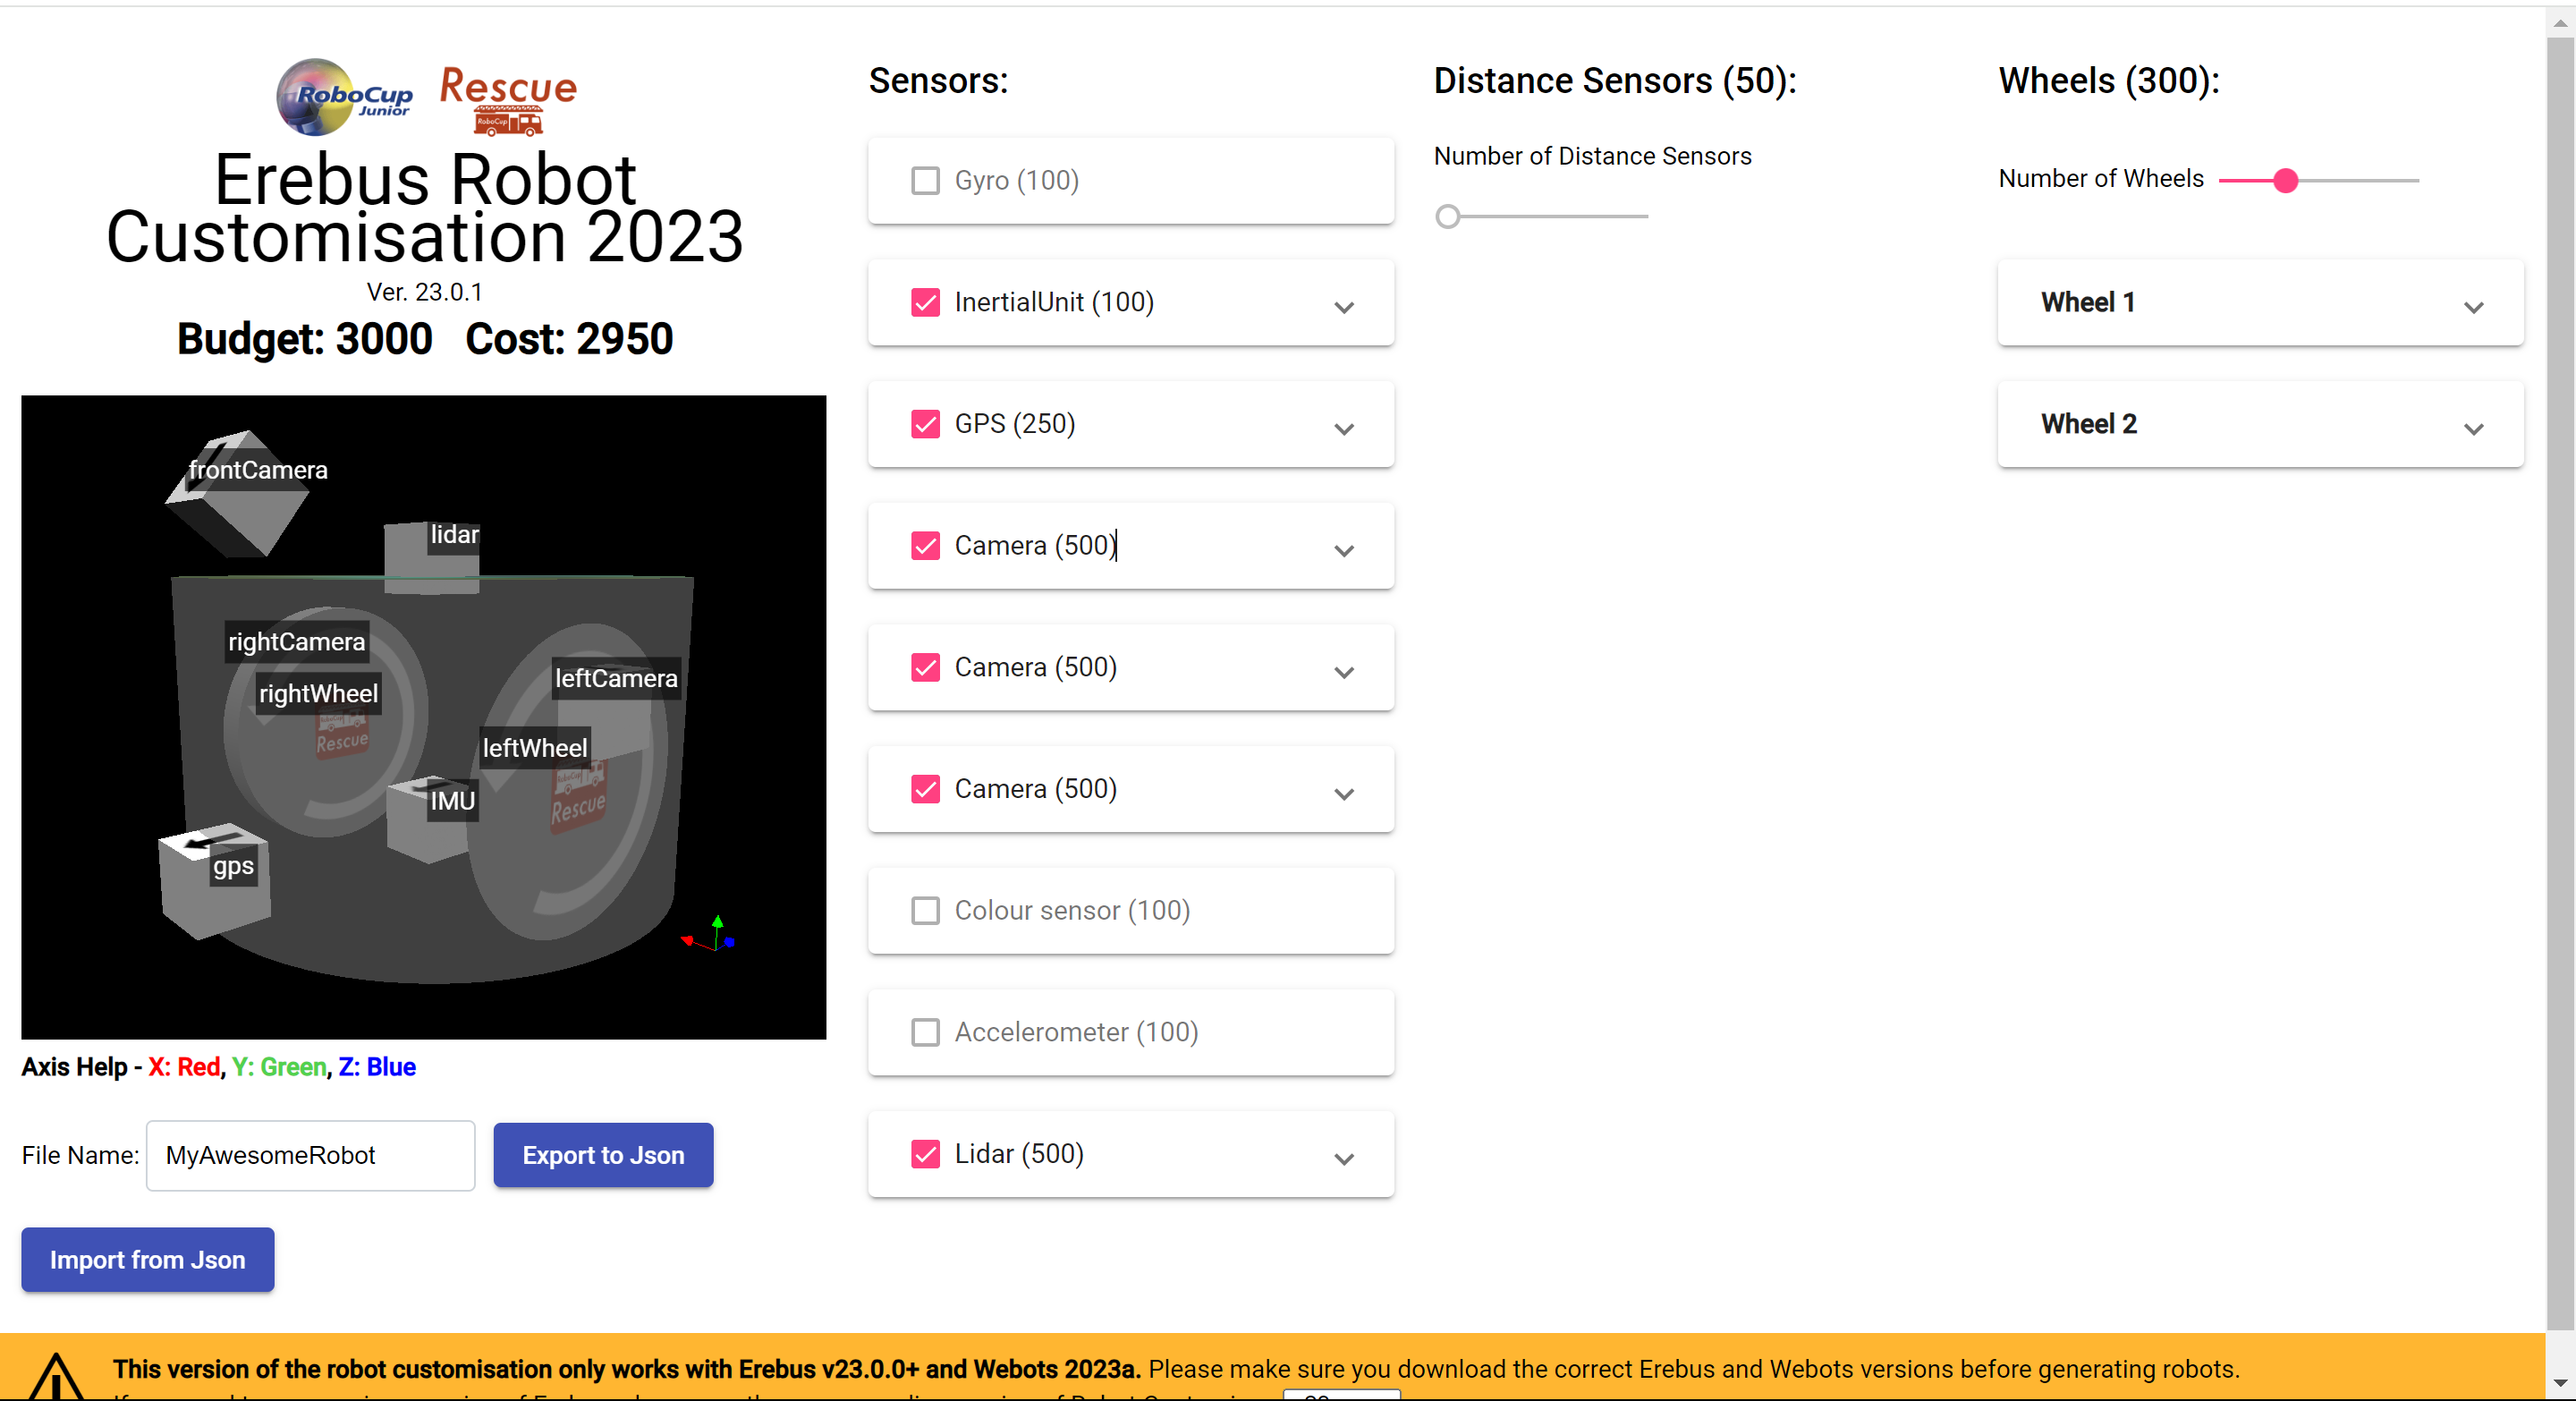
\includegraphics[width=150mm]{Photo/robot.png}

    \subsection{ロボット全般の説明}
    タイヤ・モータの数はそれぞれ2つ。Robot Customizationの標準設定をそのまま使っている。

    \subsection{使用しているセンサーと使用目的}
    \begin{itemize}
      \item 左右モータ + エンコーダ\\
      標準のものをそのまま使用している。\\
      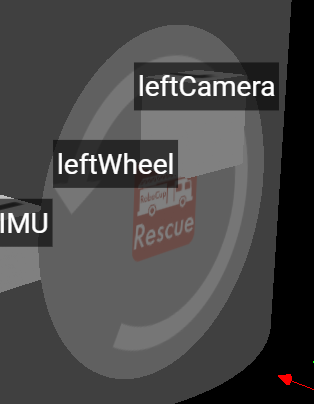
\includegraphics[width=40mm]{Photo/Parts/ダウンロード.png}
      \item IMU\\
      角度を取得するために使用している。\\
      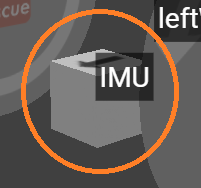
\includegraphics[width=40mm]{Photo/Parts/ダウンロード1.png}
      \item GPS\\
      位置情報を取得するために使用している。\\
      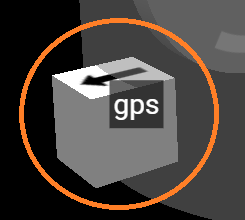
\includegraphics[width=40mm]{Photo/Parts/ダウンロード2.png}
      \item LiDAR\\
      障害物の検知、壁の認識に使用している。\\
      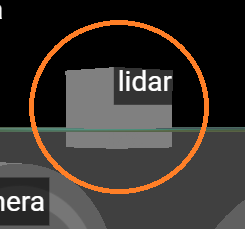
\includegraphics[width=40mm]{Photo/Parts/ダウンロード3.png}
      \item 左右カメラ\\
      被災者の検知に使用している。\\
      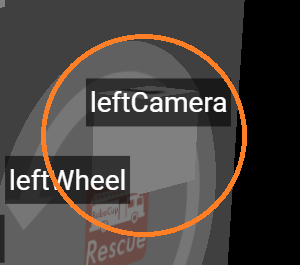
\includegraphics[width=40mm]{Photo/Parts/ダウンロード4.png}
      \item 正面カメラ\\
      障害物を発見と床の色の認識に使用している。\\
      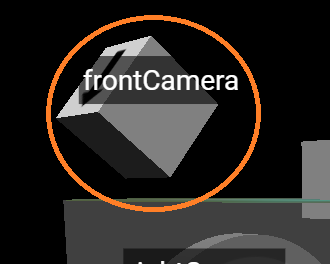
\includegraphics[width=40mm]{Photo/Parts/ダウンロード5.png}
    \end{itemize}
  
    \subsection{被災者の探索}
    \noindent
    正面と左右に1つずつカメラを搭載している。
    \vskip.5\baselineskip
    \noindent
    正面カメラ\\
    斜め上から目の前のタイル1枚を俯瞰するように設置してる。\\
    Fov(視野角)を標準の1radから1.5radに広げて使用している。
    \vskip.5\baselineskip
    \noindent
    側面カメラ\\
    被災者に対して水平な高さから、被災者がちょうど収まるくらいの位置に置いている。
  
  \section{ロボットのソフトウェア}

    \subsection{使用しているプログラミング言語・ソフトウェア}
    \noindent
    主な開発環境
    \begin{itemize}
      \item Webots 2023.a
      \item Erebus v23.0.5
      \item C++ 14 (メイン言語)
      \item Python 3.12.1
      \item Visual Studio 2022
    \end{itemize}

    使用した言語はC++である。殊レスキューシミュレーションにおいてはPythonの方がポピュラーであることは何となしに知っていたが、C++の方が好みなのでC++を採用した。\\
    もちろん、画像認識の選択肢が狭まることは承知の上である。\\

    Visual Studioの環境構築には苦労した。なにせ、レスキューシミュレーション公式サイトにもDiscordにも情報がないのである。結果的には、Webotsの公式サイトの情報を基に作成した。このままではよくないと思い、簡単にだが環境構築方法をまとめたページを作成した。\href{https://qiita.com/kikou0517/items/f13045b6b97767e7d0f0}{リンク}\\
    
    ソースコードの管理にはGitHubを使用した。draw.ioで作成したポスターと合わせて管理している。\\
    ブランチ戦略にはGitHub Flowを使用している。かつてはgit-flowを使用していたが、今回は小規模開発のためシンプルで細やかなリリースを重ねていける開発スタイルを選択した。\\
    他にも、GitHubのProject機能を使ったタスク管理を行うこともできた。\\
    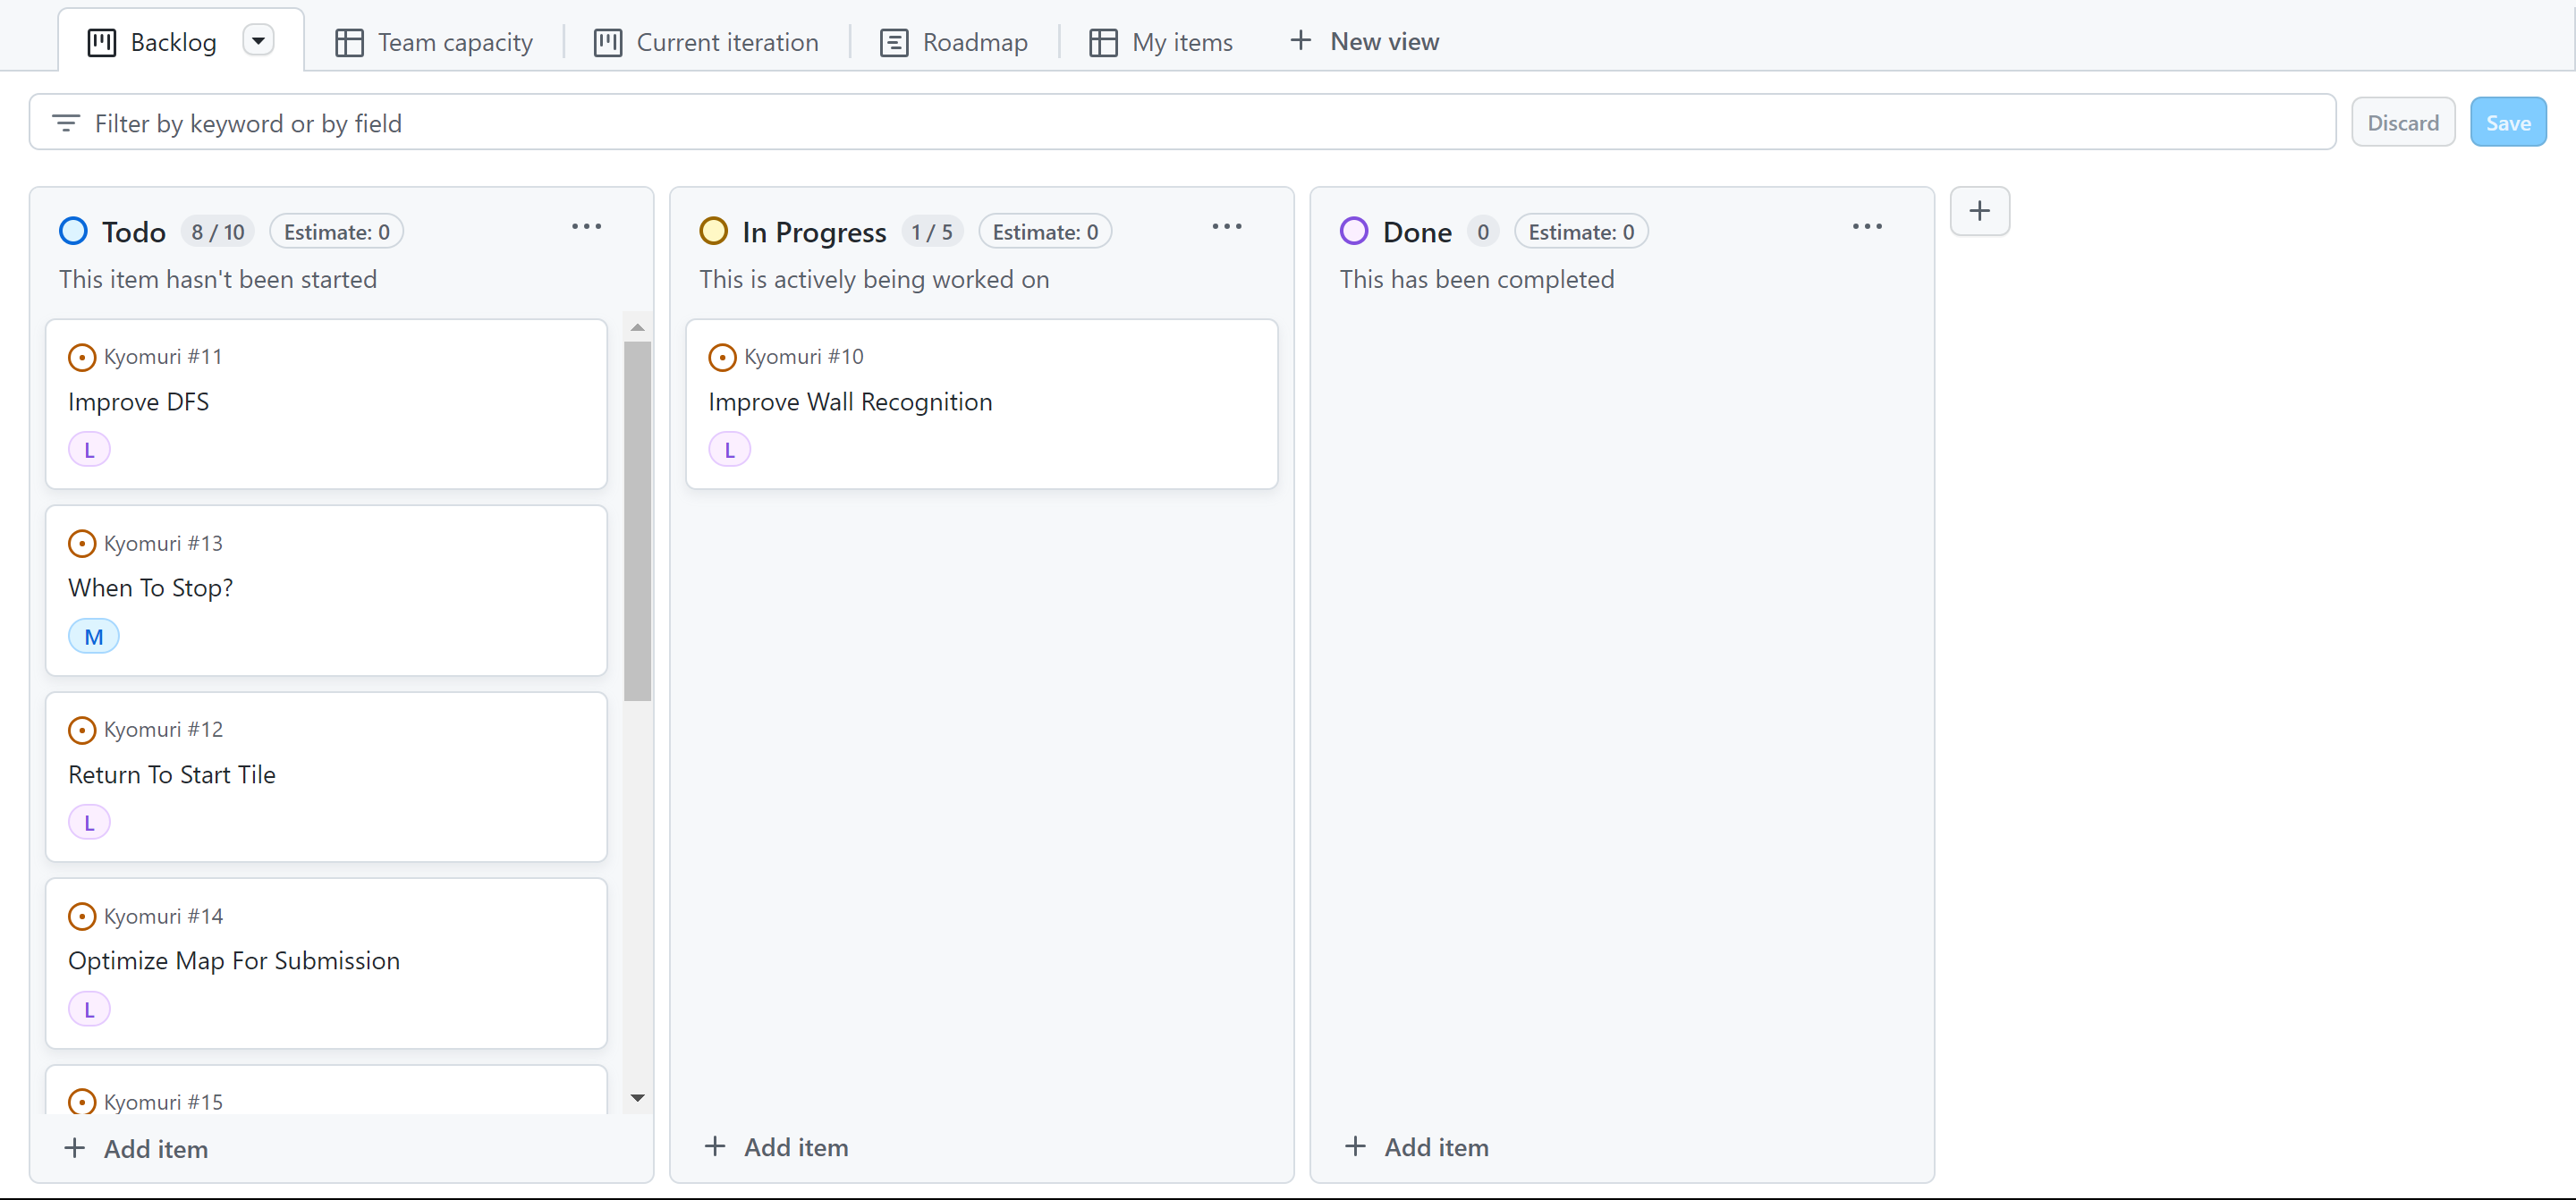
\includegraphics[width=150mm]{Photo/1.png}

    \subsection{迷路探索}

  \section{探索アルゴリズム}
  深さ優先探索を使用する。探索は6cm単位で行う。\\
  オリジナルの工夫点も加えた。\\
  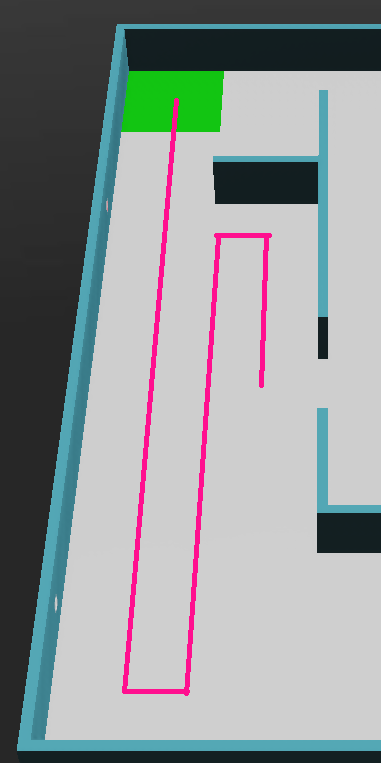
\includegraphics[width=40mm]{Photo/feagure1.png}

  上図のマップでは、ピンク線で示したように探索済みのマスを半分跨ぎながら進むという効率の悪い探索を行う可能性がある。これは機体のサイズは12$\times$12cmを基準とするのに対して、6cm単位で探索を行うことが原因である。\\
  そこで深さ優先探索における「未探索」「探索済み」という2つのパラメーターに「部分的に探索済み」を加え、進行方向の候補が複数あった場合に「部分的に探索済み」の優先度を下げることで、上図のような探索を防いでいる。\\

    \subsection{壁の認識}
    \noindent
    LiDARによる壁の認識は6cm進むごと、つまり深さ優先探索の進路選択の一部として行う。識別する方向は機体の前後左右のマスである。\\
    \noindent
    まず、ロボットが毎回完璧な位置にいるとは限らない。その影響を最小限に抑えるために2種類の補正を行う。
    \begin{enumerate}
      \item 東西南北方向に対しての傾きを補正する(下図)。修正には回転行列を用いる。\\
      $$
      \begin{pmatrix}
      X\\
      Y
      \end{pmatrix}
      =
      \begin{pmatrix}
      \cos\theta & -\sin\theta \\
      \sin\theta & \cos\theta
      \end{pmatrix}
      \begin{pmatrix}
      x\\
      y
      \end{pmatrix}
      =
      \begin{pmatrix}
      x\cos\theta - y\sin\theta \\
      x\sin\theta + y\cos\theta
      \end{pmatrix}
      $$
      \item 目標位置とのズレを補正する。こちらはズレの分だけ全ての座標をずらすだけである。
    \end{enumerate}

    \begin{figure}[H]
      \begin{minipage}[b]{0.45\linewidth}
        \centering
        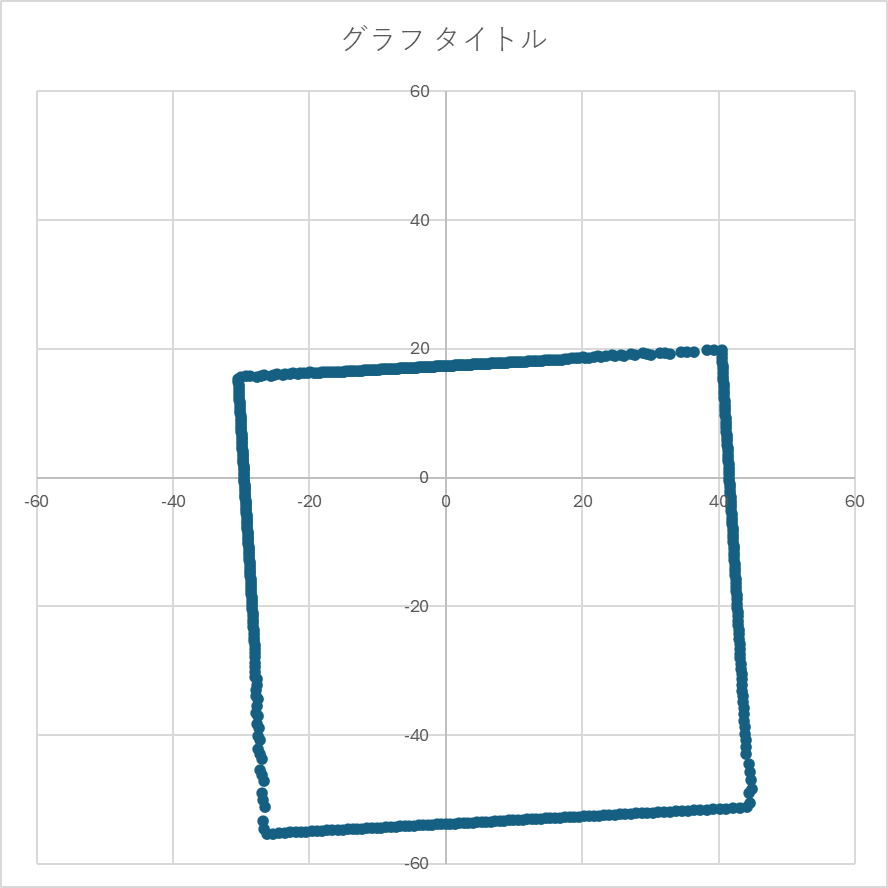
\includegraphics[keepaspectratio, scale=0.5]{Photo/image-8.png}
        \caption{修正前}
      \end{minipage}
      \begin{minipage}[b]{0.45\linewidth}
        \centering
        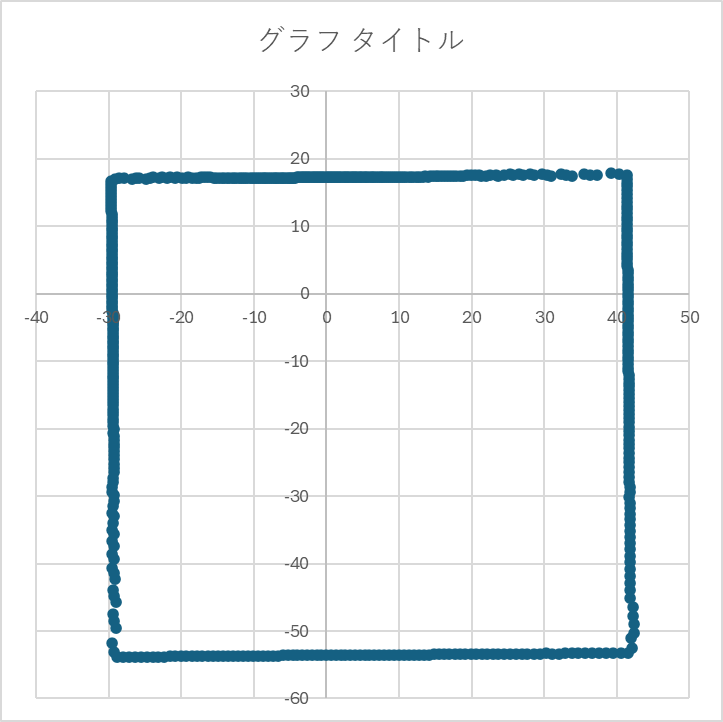
\includegraphics[keepaspectratio, scale=0.5]{Photo/image-9.png}
        \caption{修正後}
      \end{minipage}
    \end{figure}

    \noindent
    次に、壁の認識を行うのに必要な範囲のデータを切り取る。切り取る範囲はそれそれの方向の12cmである。
    \begin{figure}[H]
      \centering
      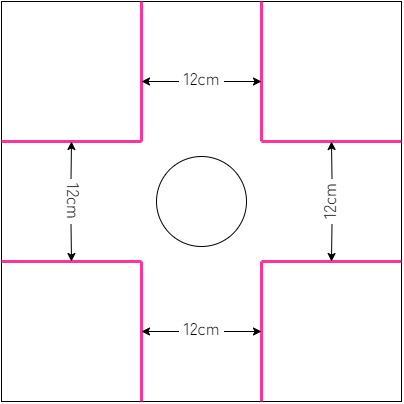
\includegraphics[width=50mm]{Photo/image2.drawio.png}
      \caption{}
    \end{figure}
    
    切り取ったデータはそれぞれの方向を向いており扱いづらいので、機体前向きに回転させる。
    \begin{figure}[H]
      \begin{minipage}[b]{0.45\linewidth}
        \centering
        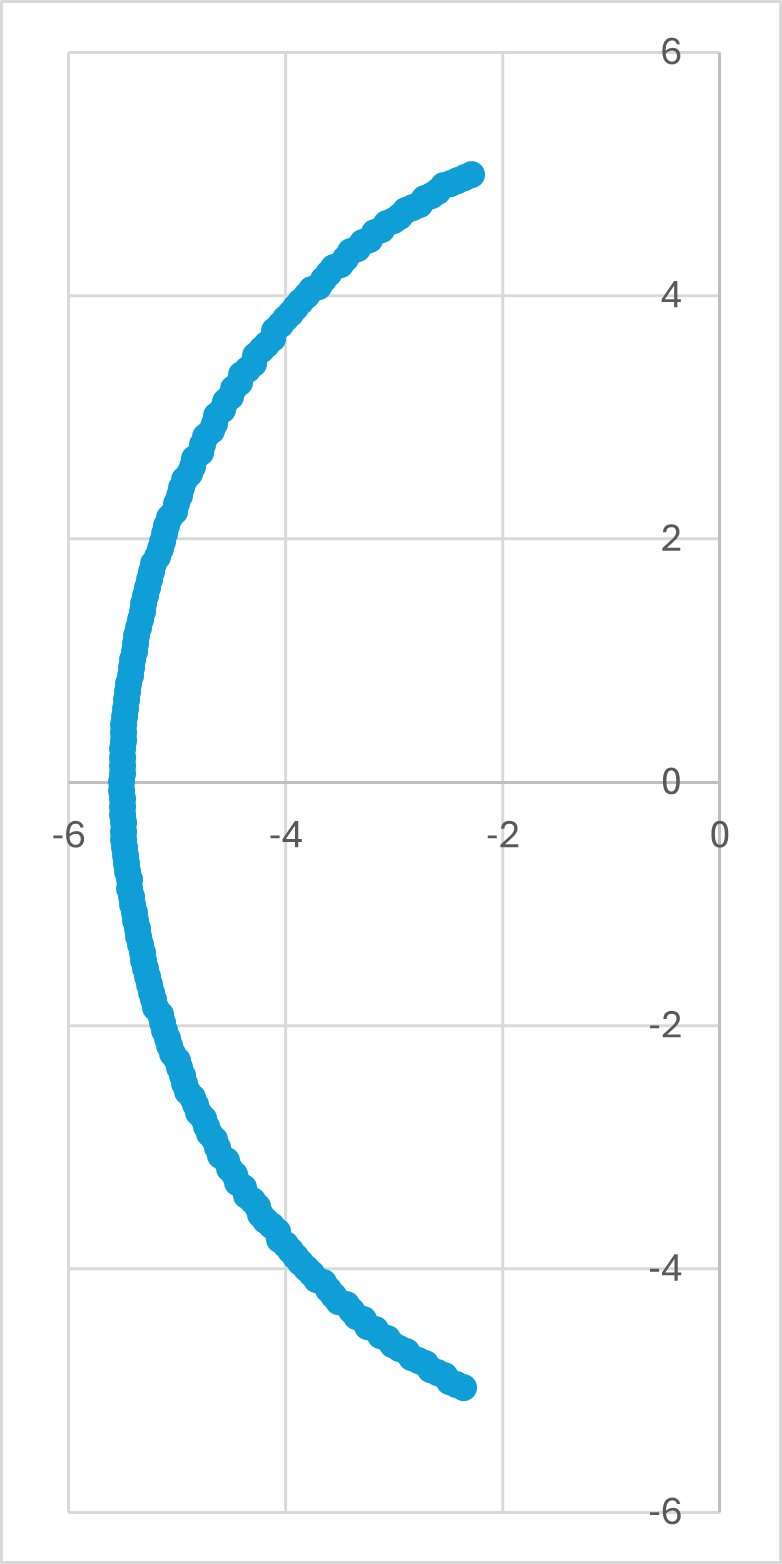
\includegraphics[keepaspectratio, scale=0.5]{Photo/画像1.png}
        \caption{修正前}
      \end{minipage}
      \begin{minipage}[b]{0.45\linewidth}
        \centering
        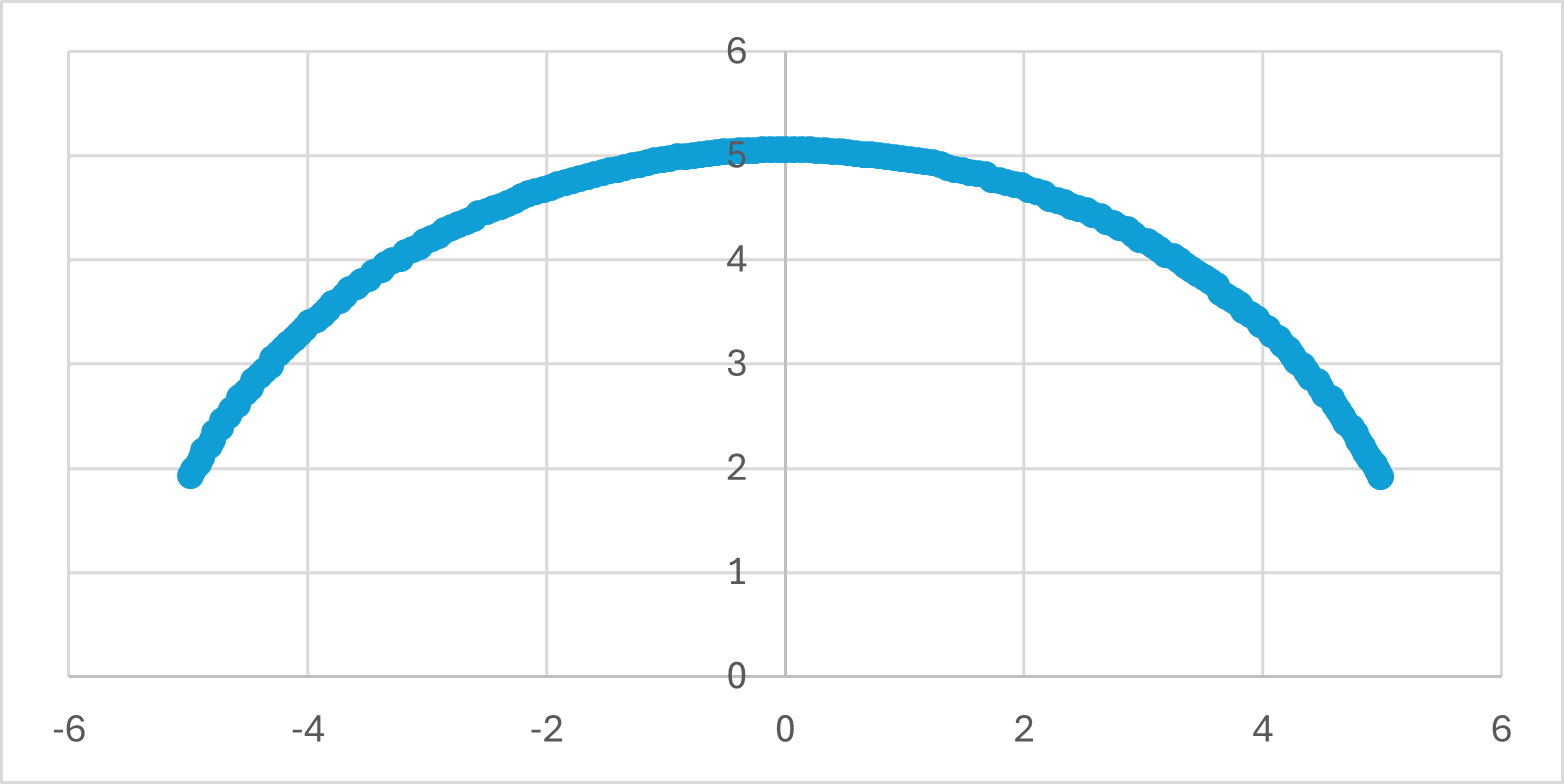
\includegraphics[keepaspectratio, scale=0.5]{Photo/画像2.png}
        \caption{修正後}
      \end{minipage}
    \end{figure}

    \subsection{障害物の検知}

  \section{アピールポイント}
    \subsection{情報公開}
    情報公開はロボカップジュニアの国是のようなもだ。\\
    しかし、シミュレーションリーグでコードをオープンにすることは、実機リーグのそれとは持つ意味合いが少し違うと考える。良くも悪くも、たった1つのexeファイルが文字通り「全て」なのだから。だが、RCJJのコミュニティに何か少しでも貢献できることがあればと思い、今年もソースコードを大会終了後に公開することにした。\\
    実際にこのソースコードを公開することで直接誰かの参考になるとはあまり思っていない。それよりも、自分を含めより多くの人が情報公開をすることで、よりコミュニティが活発になることに期待している。\\

    去年のリポジトリも公開状態だが、ポスターに明記していなかったため、アクセスする方法が限られていた。今年はポスターに載せているのでそのようなことにはならないはずである。\\
    

    \subsection{アソビゴコロ}
    ずっとカラフルな文字と黒い背景ににらめっこしていると、目だけじゃなくて心まで疲れてくる。\\
    そこでちょっとした遊び心を取り入れてみた。\\
    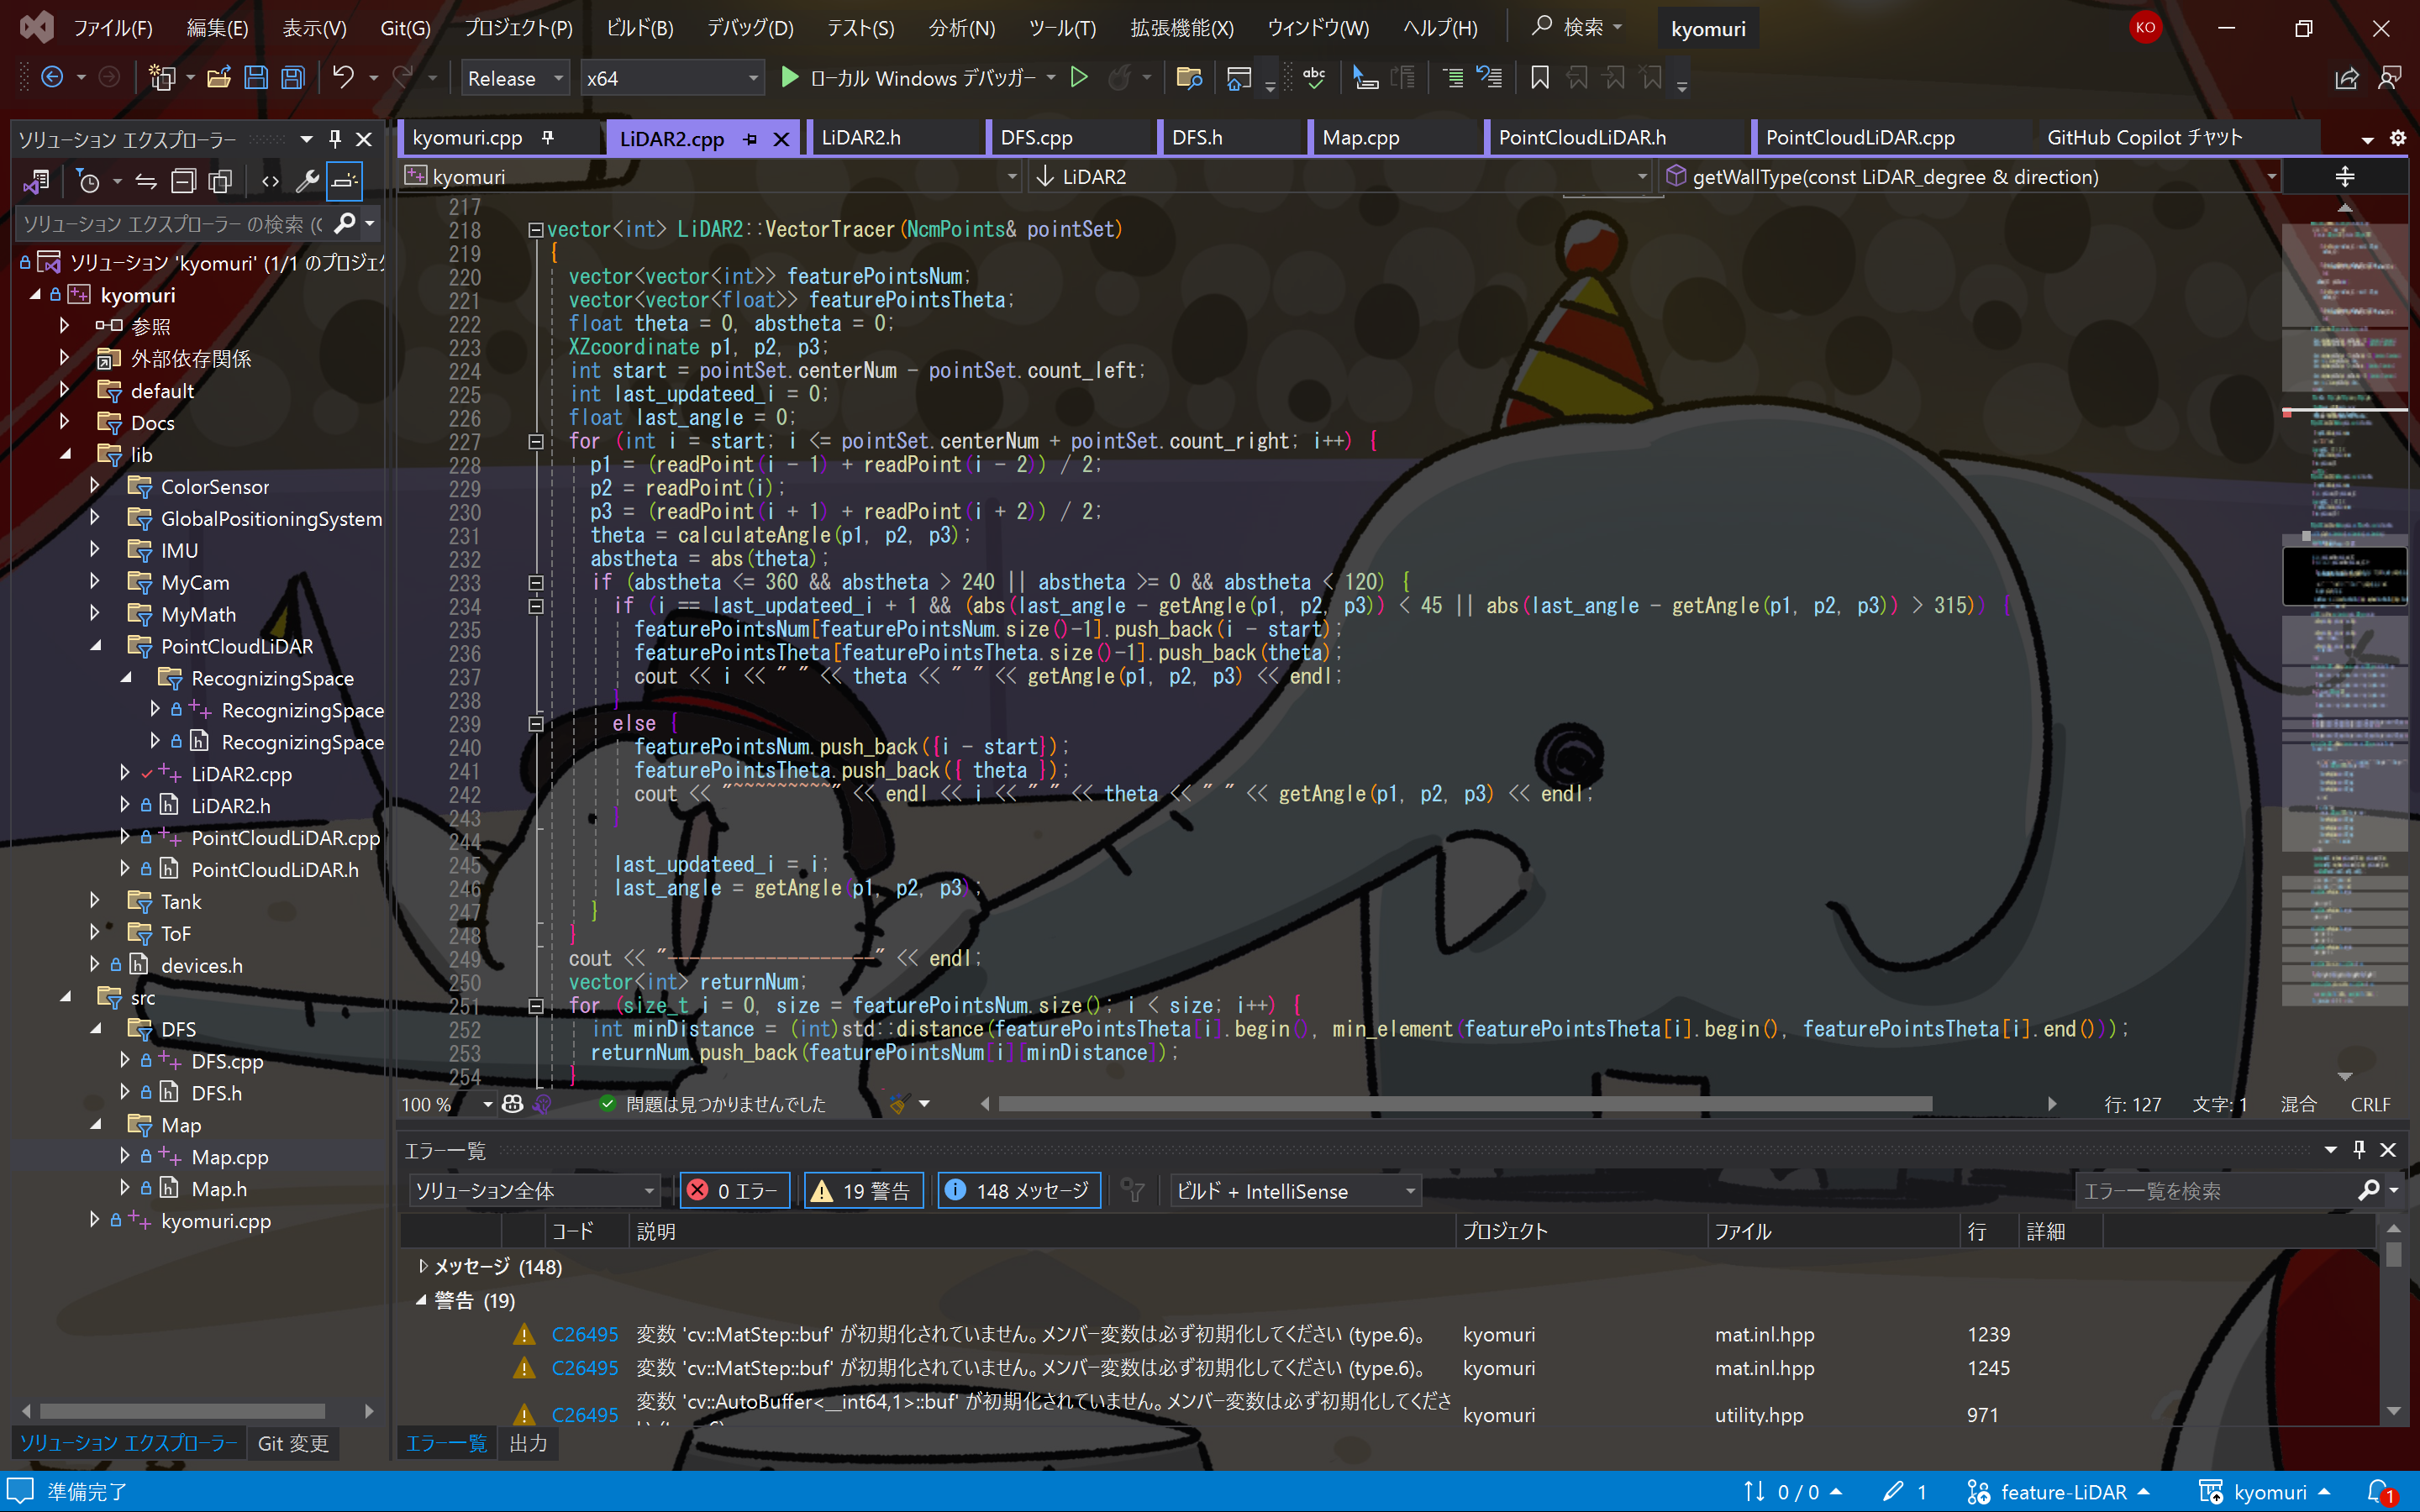
\includegraphics[width=100mm]{Photo/photo0.png}\\
    Visual Studioの画面である。見ての通り、背景にキャラクターの画像を設定している。\\

    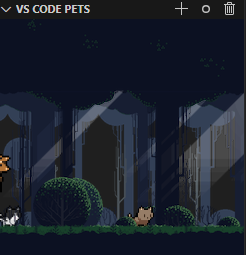
\includegraphics[width=50mm]{Photo/photo2.png}\\
    Viaual Studio Codeではvscode-petsという拡張機能を使用して、いつでも猫を眺めることができる。\\

    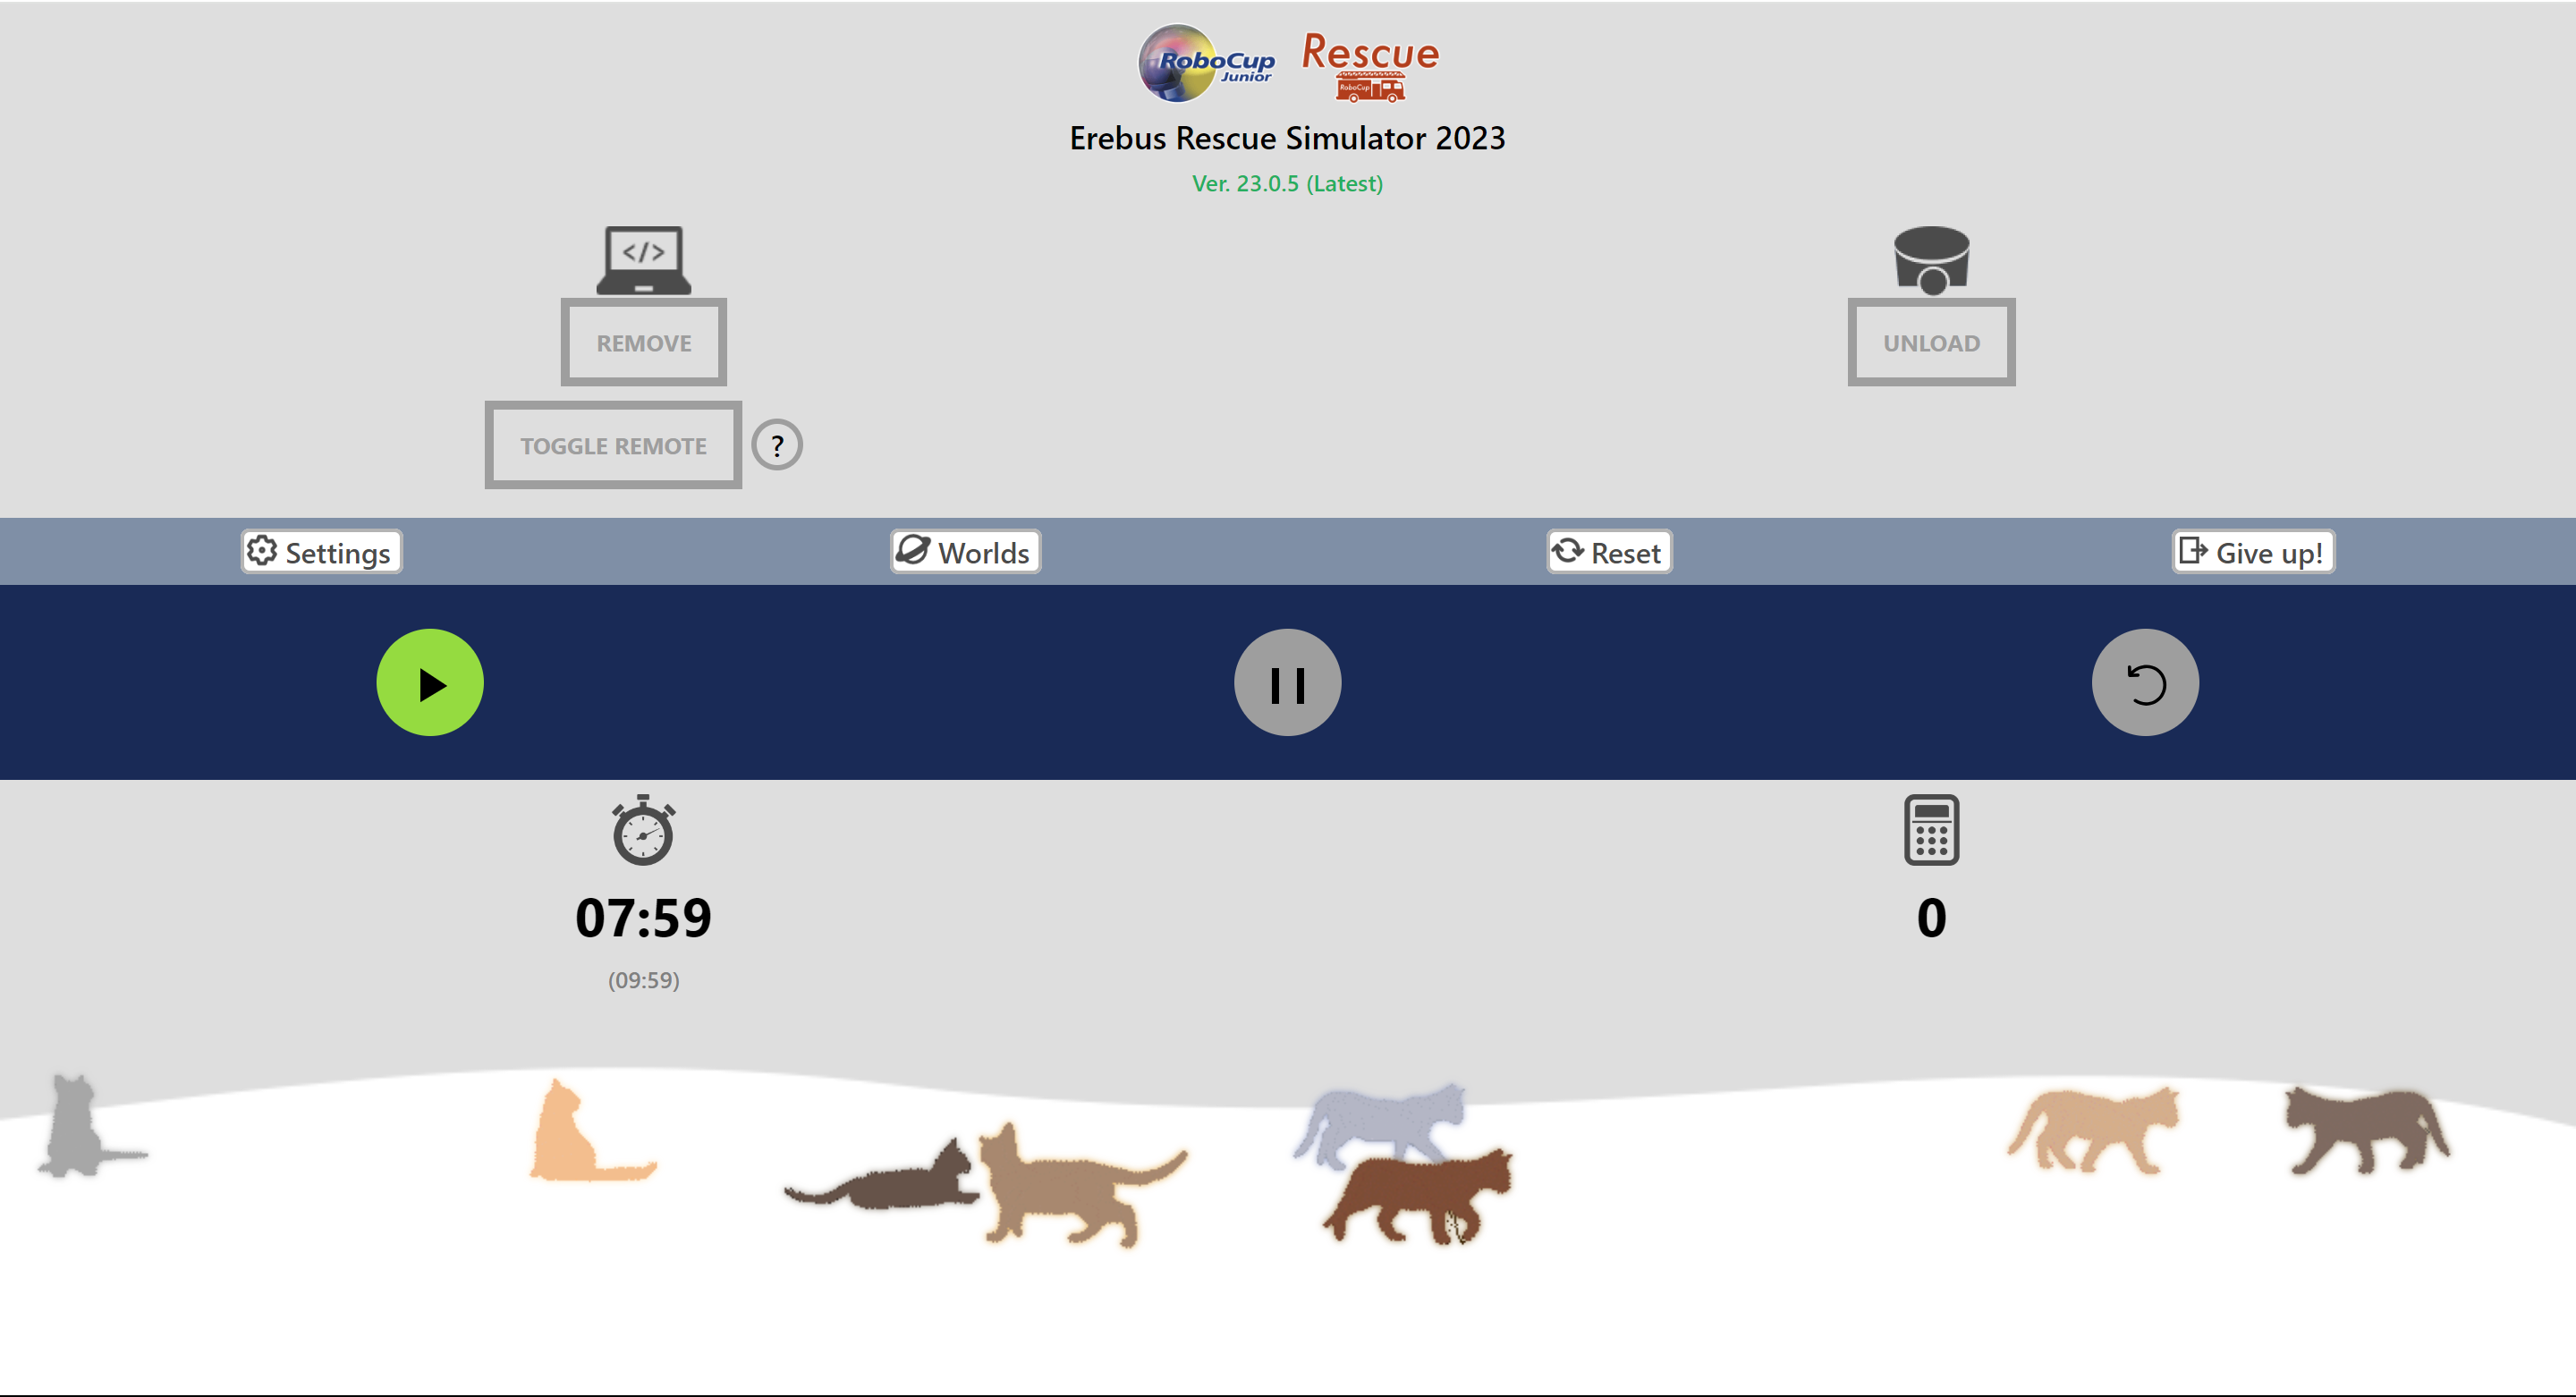
\includegraphics[width=100mm]{Photo/photo3.png}\\
    ブラウザを開けば、やはり猫がいる。"ネッコサーフィン"という拡張機能だ。\\

    こうやって、たまに癒されいている。\\


\end{document}